\documentclass{beamer}
\usepackage[utf8]{inputenc}
\usepackage[UKenglish]{babel}
\usepackage[T1]{fontenc}
\usepackage{mathtools}
\usepackage{amsmath}
\usepackage{amsthm}
\usetheme{CambridgeUS}
\usepackage{multicol}
\usepackage[margin=5pt, font={scriptsize}, labelfont={bf, it}, figurename=Rys., labelsep=space]{caption}
\usepackage[font={scriptsize}, labelfont={bf}]{subcaption}
\captionsetup{compatibility=false}

\usepackage{dsfont}
\newcommand{\1}[1]{\mathds{1}\left(#1\right)}


\newenvironment{diagrams}[2]{\begin{figure}[p]
		%\centering
		\begin{subfigure}{.49\textwidth}
			\centering
			\includegraphics[width=\textwidth]{#1.png}
			\caption{}
			\label{#1}
		\end{subfigure}
		\begin{subfigure}{.49\textwidth}
			\centering
			\includegraphics[width=\textwidth]{#2.png}
			\caption{}
			\label{#2}
		\end{subfigure}
	}
	{
	\end{figure}
}

\newenvironment{subdiagrams}[2]{
	\begin{subfigure}{.35\textwidth}
		\centering
		\includegraphics[width=\textwidth]{wykresy/#1.png}
		\caption{}
		\label{#1}
	\end{subfigure}
	\begin{subfigure}{.35\textwidth}
		\centering
		\includegraphics[width=\textwidth]{wykresy/#2.png}
		\caption{}
		\label{#2}
	\end{subfigure}
} {}

\newenvironment{subdiagram}[1]{
	\begin{subfigure}{.45\textwidth}
		\centering
		\includegraphics[width=\textwidth]{wykresy/#1.png}
		\caption{}
		\label{#1}
	\end{subfigure}
} {}


\title[Applications of Wavelets in Data Mining]{Applications of Wavelets in Data Mining}
\author[Kinga Kurowska]{Kinga Kurowska \\ supervisor: dr inż. Andrzej Giniewicz}
\date[Wrocław, \today]{Wrocław, \today}
\institute[PWr]{Faculty of Pure and Applied Mathematics \\ Wroclaw University of Science and Technology}

\begin{document}
	
\frame{\titlepage}

\begin{frame}{Table of contents}
\tableofcontents
\end{frame}

\section{Motivation}
\begin{frame}{Motivation}
\begin{block}{}
\textbf{Data Mining} is a process of automatically extracting novel, useful, and understandable patterns from a large collection of data.
\end{block}

\begin{block}{}
Wavelets could 
\begin{itemize} [<+->]
	\item provide data presentations that enable efficient and accurate mining process,
	\item be incorporated at the kernel for many algorithms...
	\item especially, in edge detection.
\end{itemize}
\end{block}
\end{frame}


\section{The main goal}
\begin{frame}{The main goal - Edge detection}
	\begin{figure}[p]
	\centering
	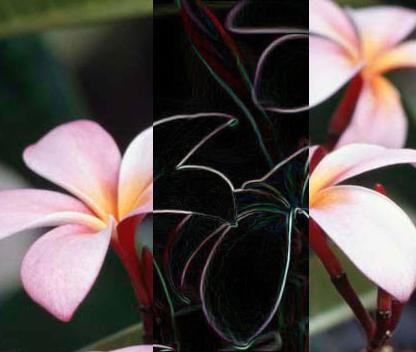
\includegraphics[width=0.7\textwidth]{edges.jpg}
	\end{figure}
\end{frame}


\section{Wavelets theory}
\subsection{What is a wavelet?}
\begin{frame}{What is a wavelet?}
The term \textbf{wavelet} means a \textbf{small wave}:
\begin{itemize}
	\item wave - the function is oscillatory,
	\item smallness - the function is of finite length or compactly supported.
\end{itemize}


A \textbf{mother wavelet} is a function
$\psi(x)$ such that
$$\{\psi(2^jx - k),\ i, k \in Z\}$$
is an orthonormal basis of $L^2(R)$.

\begin{block}{}
The term mother implies that the functions with different regions of support that are used in the transformation process are derived by dilation and translation of the mother wavelet.
\end{block}
\end{frame}

\begin{frame}{The most popular mother wavelets}
	\begin{figure}[p]
		\centering
		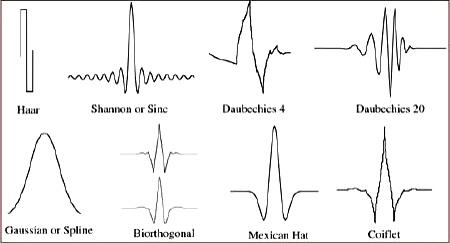
\includegraphics[width=0.9\textwidth]{wavelet_samples.jpg}
	\end{figure}
\end{frame}


\begin{frame}{Dilation Equation - How to find the wavelets?}
The key idea is self-similarity. Start with a function
$\phi(x)$ that is made up of smaller version of itself. This is the dilation equation 
$$
\phi(x) = \sum_{k=-\infty}^{\infty} a_k \phi(2x - k),
$$
where $a_k$'s are called filter coefficients or masks. The function $\phi(x)$ is called \textbf{the scaling function (or father wavelet)}. 

Under certain conditions, the formula below gives a wavelet.
$$
\psi(x) = \sum_{k=-\infty}^{\infty} (-1)^k a_k \phi(2x - k)
$$
\end{frame}


\subsection{Wavelet transform}
\begin{frame}{Wavelet transform}

%\begin{block}{}
%	Generally speaking, the wavelet transform is a
%	tool that partitions data, functions, or operators into different frequency components
%	and then studies each component with a resolution matched to its
%	scale.
%\end{block}

\begin{block}{Why bother to have wavelets if they are very much the same as Fourier transforms
except they have different bases?}

Wavelet transform is capable of providing \textbf{time and frequency localizations
simultaneously} while Fourier transforms could only provide frequency representations.
Fourier transforms are designed for stationary signals because they
are expanded as sine and cosine waves which extend in time forever.
\end{block}

\begin{block}{}
	Fourier transform is not suitable for non-stationary signal with time varying frequency.
\end{block}
\end{frame}

\begin{frame}{Fourier transform vs Wavelet transform}
	\begin{figure}[p]
		\centering
		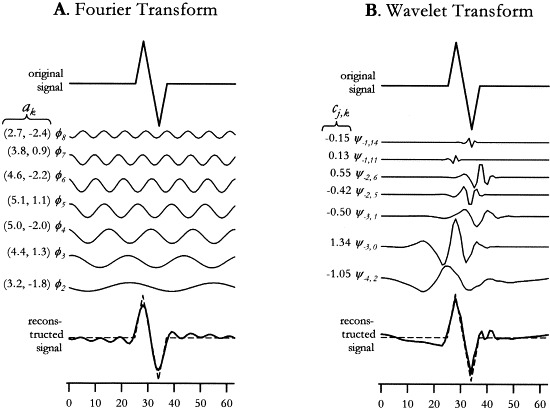
\includegraphics[width=0.7\textwidth]{FTvsWT.jpg}
	\end{figure}
\end{frame}

\subsection{Properties of Wavelets}
\begin{frame}{Properties of Wavelets}
\begin{itemize} [<+->]
	\item \textbf{Computational Complexity}: Fast wavelet transform only needs $O(N)$ multiplications. The space complexity is also linear. To compare, discrete Fourier transform requires $O(N^2)$ multiplications and fast Fourier transform also needs $O(N log (N))$ multiplications.
	
	\item \textbf{Vanishing Moments}: A function $f (x)$ which is supported in bounded region $w$
	is called to have $n$-vanishing moments if it satisfies the following equation:
	$\int_w f(x)x^j dx = 0,\ j = 0,1,\ldots,n$. For example, Haar wavelet has 1-vanishing
	moment and $db2$ has 2-vanishing moment. The intuition of vanishing moments
	of wavelets is the \textbf{oscillatory nature} which can thought to be the characterization
	of difference or details between a neighborhood of the data.
	
\end{itemize}
\end{frame}

\begin{frame}{Properties of Wavelets}
\begin{itemize} [<+->]
	\item \textbf{Compact Support}: Each wavelet basis function is supported on a finite
	interval. Compact support guarantees the localization of wavelets - processing a region of data with wavelet does not affect the data out of this region.
	
	\item \textbf{Decorrelated Coefficients}: Wavelets reduce temporal correlation so that the correlation of wavelet coefficients are much smaller than the correlation of the corresponding temporal process. Hence, the wavelet transform could be used to reduce the complex process in the time domain into a much simpler process in the wavelet domain.
	
	\item There are also some other favorable properties of
	wavelets such as the \textbf{symmetry} of scaling and wavelet functions, \textbf{smoothness}
	and the availability of \textbf{many different wavelet basis functions}.
\end{itemize}
\end{frame}


\section{Edge detection}
\begin{frame}{Edge detection}
\begin{block}{}
	\textbf{Edges} can be considered as transients in a signal or mathematically defined as local singularities. 
	In practice, edges are points in an image where brightness changes suddenly.
\end{block}
	
\begin{block}{}
	\textbf{Edge detection} refers to the process of identifying and locating sharp
	discontinuities in an image. In wavelet edge detection technique, the is used \textbf{Discrete Wavelet Transform} (DWT) and the filter is one which searches for the local maxima in a wavelet domain.
\end{block}
\end{frame}

\subsection{2-D Discrete Wavelet Transform}
\begin{frame}{2-D Discrete Wavelet Transform}
The 2D algorithm is based on separate variables leading to prioritizing of $x$ and
directions. The scaling function is defined by
$$
\phi(x, y) = \phi(x) \phi(y).
$$

The detail signal is obtained from three wavelets:
\begin{itemize}
	\item a vertical wavelet: $\psi^1(x, y) =\phi(x)\psi(y)$,
	\item a horizontal wavelet: $\psi^2(x, y) = \psi(x) \phi(y)$,
	\item a diagonal wavelet: $\psi^3(x, y) = \psi(x) \psi(y)$.
\end{itemize}
which leads to three sub-images in each of the decomposition levels.
\end{frame}

\begin{frame}{2-D DWT Coefficients}
	\begin{figure}[p]
	\centering
	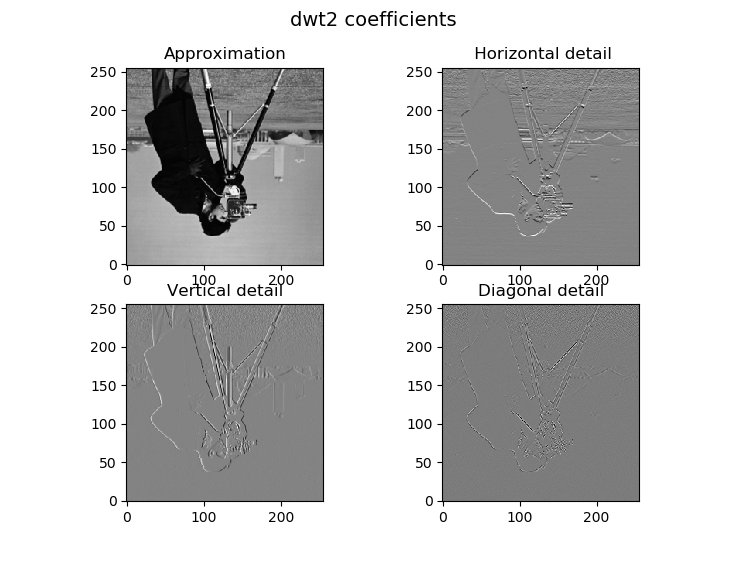
\includegraphics[width=0.8\textwidth]{dwt2_coefficients.png}
\end{figure}
\end{frame}


\begin{frame}{Thresholding}
	\begin{figure}[p]
		\centering
		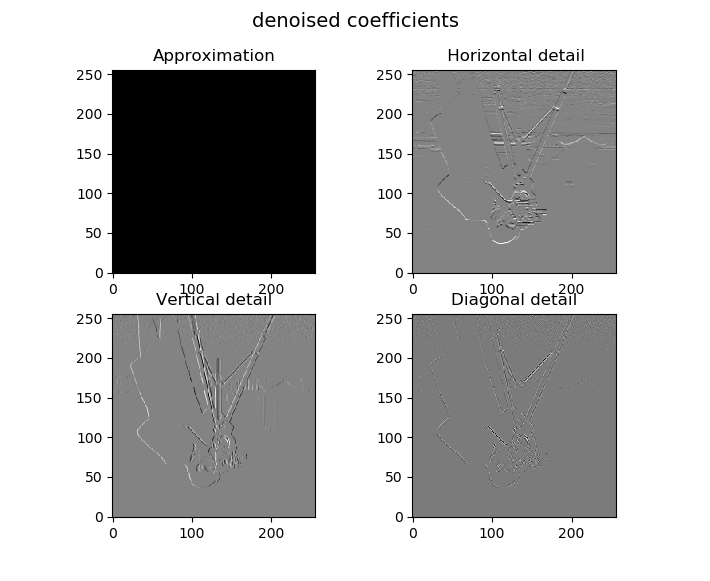
\includegraphics[width=0.8\textwidth]{denoised_coefficients.png}
	\end{figure}
\end{frame}


\begin{frame}{Inverse DWT}
\begin{diagrams}{original}{edges_detected}
	\centering
\end{diagrams}
\end{frame}

\section{Bibliography}
%[allowframebreaks]
\begin{frame}{Bibliography}
\begin{thebibliography}{9}
	\beamertemplatearticlebibitems
	\bibitem{WaveletMethodsInDataMining}
	T. Li, S. Ma,  M. Ogihara, ''Wavelet methods in data mining'', Data Mining and Knowledge Discovery Handbook (2005): 603-626,
	
	\bibitem{WaveletSupportVectorMachine}
	L. Zhang, W. Zhou, L. Jiao, ''Wavelet support vector machine'', IEEE Transactions on Systems, Man, and Cybernetics, Part B (Cybernetics) 34.1 (2004): 34-39,
	
	\bibitem{EdgeDetection}
	Chesnokov Yuriy, ''Edge Detection in Images with Wavelet Transform'', website: www.codeproject.com, 14 Nov 2007,
	
	\bibitem{citekey}
	V. R. Chaganti, ''Edge Detection of Noisy Images Using 2-D Discrete Wavelet Transform'', 2005.
	
%	\beamertemplatebookbibitems
%	\bibitem{Lehmann1968}
%	E. L. Lehmann. ,,Testowanie hipotez statystycznych''. PWN, 1968.
	
\end{thebibliography}
\end{frame}

\end{document}
